\documentclass[9pt,twocolumn,twoside]{../../styles/osajnl}
\usepackage{fancyvrb}
\journal{i524} 

\title{Allegro Graph}

\author[1,*, +]{Diksha Yadav}

\affil[1]{School of Informatics and Computing, Bloomington, IN 47408, U.S.A.}

\affil[*]{Corresponding authors: yadavd@umail.iu.edu}

\affil[+]{HID - S17-IR-2044}

\dates{Paper-001, \today}

\ociscodes{Allegro, Graph, triples, SPARQL, RDF}

% replace this with your url in github/gitlab
\doi{\url{https://github.com/diksha2112/sp17-i524/tree/master/paper1/S17-IR-2044/report.pdf}}


\begin{abstract}
Allegro Graph is a database technology that turns complex data into actionable business insights.
It is a database technology that is used for analyzing complex information with relationships in the data which cannot be represented or analyzed by traditional database technologies. So, when our data contains relationships in it, we cannot use traditional database. We have use some advanced technology, one of which is "Allegro Graph".

\end{abstract}

\setboolean{displaycopyright}{true}

\begin{document}

\maketitle

\section{Introduction}
As stated by the developer of AllegroGraph, “Franz”, “AllegroGraph is a database technology that enables businesses to extract sophisticated decision insights and predictive analytics from their highly complex, distributed data that can’t be answered with conventional databases, i.e., it turns complex data into actionable business insights.” \cite{fag}
It can be viewed as a closed source database that is used for storage and retrieval of data in the form of triples (triple is a data entity composed of subject-predicate-object like “Professor teaches students”). 

Information in a triplestore is retrieved using a query language. Query languages can be classified into database query languages or information retrieval query languages. The difference is that a database query language gives exact answers to exact questions, while an information retrieval query language finds documents containing requested information. \cite{wag}

Triple format represents information in a machine-readable format. Every part of the triple is individually addressable via unique URLs — for example, the statement “Professor teaches students” might be represented in RDF(Resource Description Framework ) as http://example.namehashProfessor12http://xmlns.com/foaf/0.1/teacheshttp://example.namehashstudents. Using this representation, semantic data can be queried and reasoned unambiguously \cite{str}

\section{Architecture}
AllegroGraph has the REST protocol architecture which is a superset of the Sesame HTTP Client. Adapters for various languages including Sesame Jena, Sesame Java, Python using the Sesame signatures, and Lisp are supported. Other than this, Open Source Adapters for Csharp, Clojure, Ruby, Scala, and Perl are available. We can view the architecture of AllegroGraph in visualization 1 \cite{fag}

\begin{figure}[htbp]
	\centering
	\fbox{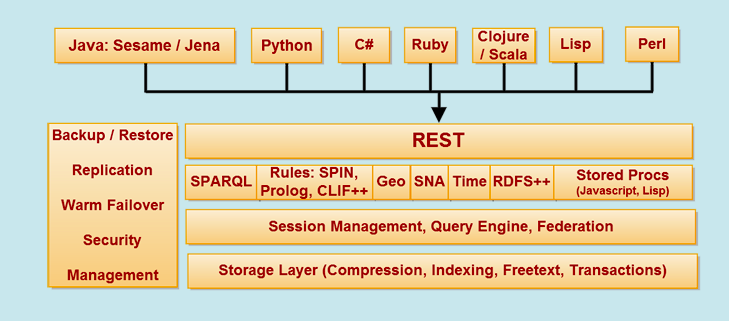
\includegraphics[width=\linewidth]{images/arch.png}}
	\caption{Allegro Graph Architecture}
	\label{fig:Allegro-arch}
\end{figure}

\section{Features}
1) RDF-Structure of data is maintained while exchange of information.

2) SPARQL-It is the standard query language used for writing complex structured, semi-structured or semi structured queries. It works excellently for changing databases or databases in which relationship is included in data.

3) Advanced queries-Advanced queries can be run on Allegro graph that cannot be executed by conventional relational databases and even difficult to execute with Hadoop like Geospatial (location), Temporal (time difference), Social Networking (relationships) and library (activities).

4) Linked Open Data-Allegro graph has the ability to link to the data elements of a large number of
Publically- published semantic graph databases.

5) ACID Database model-Allegro graph adheres to full ACID database model and data integrity.

6) Magic predicates-Allegro graph uses predicates for better representation of real world which is helpful in processing of complex data and better predictions in business.

7) String support-Unlimited length is available for data elements to support lengthy URL references

8) Dereferenceable URLs-Reach of graph is extended to other database sources. So, entire web can be leveraged as information sources linked by graphical databases.

9)  Enterprise Platform- Graph databases needs enterprise platform features (Enterprise scale, ACID, commit, roll-back, triple level security model, Cloud enabled, checkpoint, replication, auditing) to be reliable, robust and for high availability.

10) Cloud and on premise licensing- AllegroGraph has flexibility to run locally or from Amazon Web Services (AWS) whatever option suits the business and technical needs.

11) Predictive Analysis-AllegroGraph provides a unique and powerful platform for predictive analysis with combination of graph, semantics, rules/logic, geospatial, temporal, social networking etc.

12) Event Support-Supports for events in which machine learning is required along with other features of AllegroGraph.

13) HDFS file system support- Supports loading of files from Hadoop Distributed File System.

14) Compatible Semantic Technologies-AllegroGraph is compatible with several semantic technologies-
like Data maestro, Talend, Callimachus, TopBraid Composer, Gruff, MongoDB, Solr, Semaphore, Allegro Set, Linked data, Racer Pro, Sentient Suite, KnowMed, Cogito etc \cite{fag}

\section{System Requirements}
The AllegroGraph database server runs on Linus x86-64 bit. To run AllegroGraph on other operating systems (i.e. Windows, Mac) Linux Virtual Machine or EC2 must be set up.
\cite{fag}

\section{Benefits}
1)AllegroGraph semantic graph technology can automatically link new information irrespective of the format of the information. No manual user intervention is required for analysis of structure and relationships in information. Also, there is no need to pre structure the database.

2)Since AllegroGraph uses self-defined and schema less data, it is able to structure the new information automatically when it is ingested into AllegroGraph. So, if we have several databases, then automatic linking of data of all the databases can be done powerfully by AllegroGraph without any user intervention. For this task to take place in conventional relational databases, complex coding, pre-processing, data warehousing and expert knowledge of queries is required \cite{fag}

\section{Popularity(Allegro Graph Vs Blazegraph)}
Popularity of allegro graph in comparison to other similar technology can be seen from following plot by DB Engines ranking,

\begin{figure}[htbp]
	\centering
	\fbox{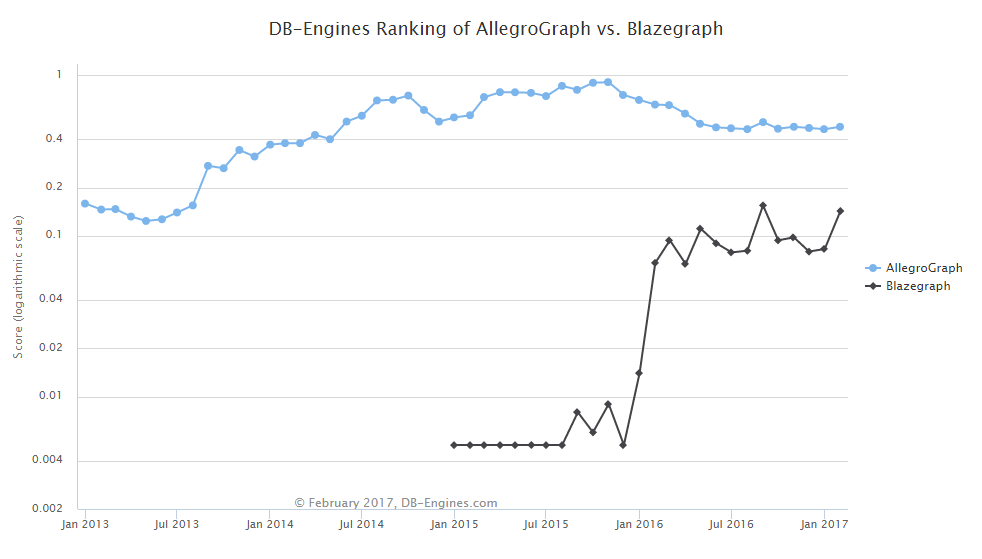
\includegraphics[width=\linewidth]{images/pop.png}}
	\caption{Allegro Graph Popularity}
	\label{fig:Allegro-Popularity}
\end{figure}
\cite{dbe}

\section{Resources for learning Allegro Graph}
Allegro graph tutorial:

http://franz.com/agraph/support/documentation/current/agraph-tutorial.html

\cite{tut}

\section{Acknowledgement}
I thank Franz, the developer of AllegroGraph for information on Allegro graph published on their website. I am also grateful to Dr. Gregor von Laszewski for providing the appropriate paper template.


\section{Conclusion}
Since Allegro Graph makes it easier for the users to analyze complex information using graphical format without much necessity for manual intervention, its popularity and utilization is increasing with time as compared to similar database technologies.


% Bibliography

\bibliography{references}

\end{document}
